Vi har i løpet av prosjektet produsert en prototype på en koblingsagent som skal fungere som en illustrering på hvordan en generell og enkel koblingsagent kan fungere i praksis. Prototypen fokuserer på å demonstrere hvor enkelt en slik koblingsprosess kan foregå, fremfor å bruke tunge, avanserte koblingsalgoritmer. Videre vil vi bruke også benytte begrepet ``matching'' mellom giver og mottaker da dette bedre beskriver vår bruk av koblingsagenten.

Årsaken til at vi valgte å implementere en koblingsagent basert på få og enkle parametere var rammene rundt problemstillingen. I matchingen mellom mottakere og givere i forbindelse med ``Gi bort dagen'' er ikke poenget å få til de mest avanserte matchingene, men snarere å gi en automatisk match basert på noen få viktige kriterier. En enkel matching er nok til å gjøre ``Gi bort dagen'' skalerbar, i tillegg til å gjøre det fremtidige ideelle selskapet ``Good Stuff'' bærekraftig.

En enkel koblingsagent vil dessuten bli mer generell, slik at det er mulighet for å benytte den i andre forbindelser enn ``Gi bort dagen''. På denne måten har koblingsagenten mulighet til å bidra til alternative forretningsideer for ``Good Stuff''.

\section{Presentasjon av koblingsprosessen}

Brukervennlighet har vært viktig i utvikling av prototypen. Nedenfor vil koblingsprosessen, fra registrering av organisasjon til presentasjon av mulige matcher, bli presentert fra brukererens perspektiv. I og med at prosessen er nær sagt identisk for mottaker og giver, vil vi kun presentere prosessen sett fra givers perspektiv. Den eneste forskjellen mellom mottaker og giver er valget mellom å motta eller bidra slik at de tekstlige meldingene brukeren ser er noe ulike.\\

Koblingsprosessen består av fem steg.\\

\newpage

{\bf Steg 1:} Velg om din bedrift ønsker å bidra eller motta.
\begin{center}
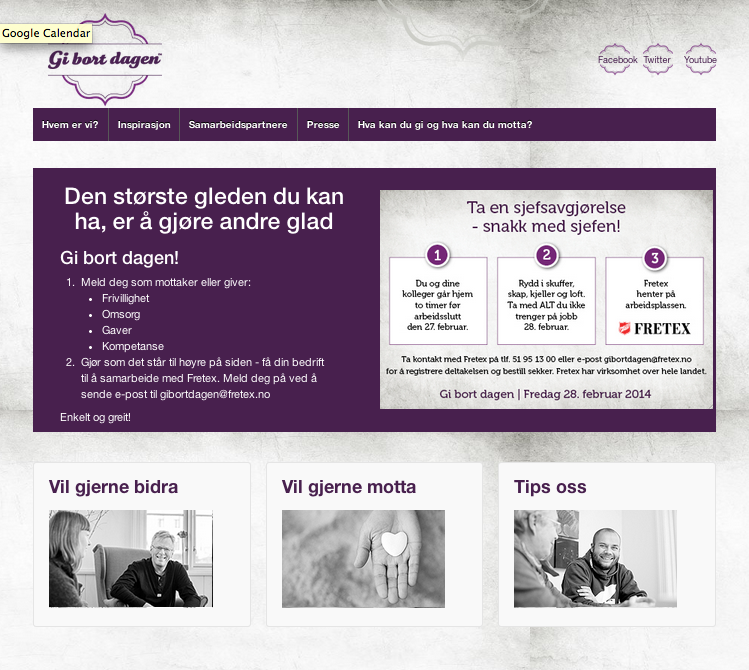
\includegraphics[clip=true, width=1 \textwidth,
trim=0cm 0cm 0cm 0cm]{startside.png}
\captionof{figure}{Protoypens startside}
\label{fig:startside}
\end{center}

Det første valget du blir stilt ovenfor når din bedrift har bestemt seg for at de skal delta på “Gi bort dagen” er om du vil delta som bidragsyter eller mottaker. Dette indikerer du på prototypens startside ved å trykke på enten ``Vil gjerne bidra'' eller ``Vil gjerne motta''. Det er også mulig å tipse om potensielle mottakere ved å trykke på ``Tips oss''.\\

\newpage

{\bf Steg 2:} Registrer bruker (giver eller mottaker)
\begin{center}
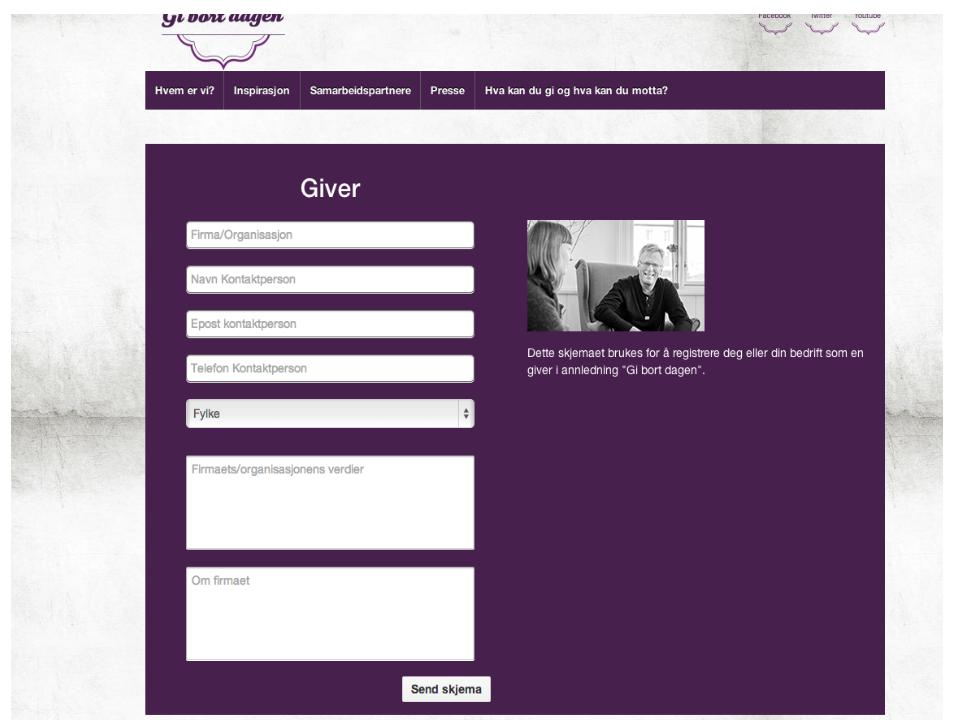
\includegraphics[clip=true, width=1 \textwidth,
trim=0cm 0cm 0cm 0cm]{registreringavbruker.jpg}
\captionof{figure}{Registrering av giver i prototypen}
\label{fig:registrering}
\end{center}

Når en giver eller mottaker registrerer seg i databasen må brukeren fylle inn kritisk informasjon som firmanavn, navnet på, epost adressen til og telefonnummer til bedriftens kontaktperson, samt bedriftens lokasjon i form av fylke. I tillegg må brukeren fylle inn firmaets/organisasjonens verdier dersom de har det, og skrive en kort beskrivelse om firmaet. Når alle nødvendige punker er fylt ut må brukeren trykke på ``Send skjema'' for å komme videre i prosessen.\\

\newpage

{\bf Steg 3:} Valg av hva bedriften vil gi eller motta
\begin{center}
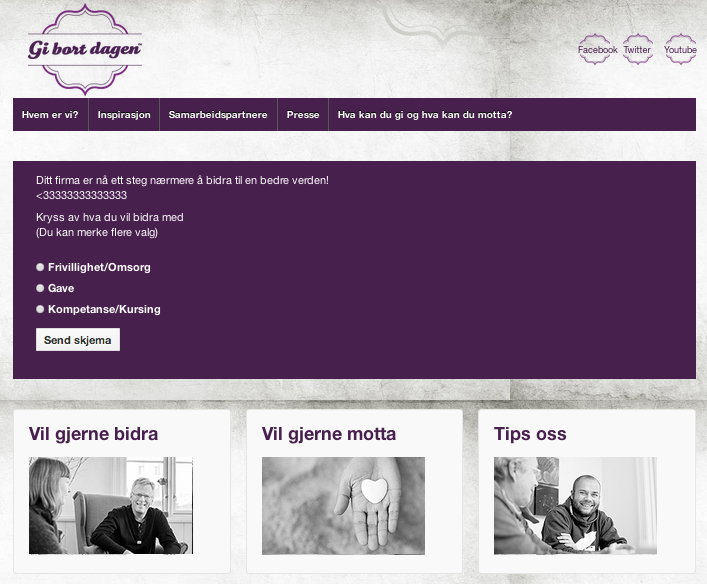
\includegraphics[clip=true, width=1 \textwidth,
trim=0cm 0cm 0cm 0cm]{valg1.png}
\captionof{figure}{Prototypens valg av hva giver vil bidra med}
\label{fig:bidra}
\end{center}

Etter at du har registrert deg som giver eller mottaker må du velge hva du ønsker å bidra med eller motta. Du vil i denne sammenhengen ha tre valgmuligheter:\\

\begin{itemize}
    \item Frivillighet/Omsorg
    \item Gave
    \item Kompetanse/Kursing
\end{itemize}
Et eksempel på frivillighet/omsorg kan være å hjelpe til på et suppekjøkken. En gave kan blant annet være en PC eller en konsert. Kompetanse/kursing kan f.eks. være spanskopplæring. Når brukeren har valgt en av kategoriene må han/hun trykke på ``Send skjema'' for å komme videre.\\

\newpage

{\bf Steg 4:} Spesifiser tema innenfor kategorien valgt i steg 3.\\
Tre ulike skjemaer vil derfor vises avhengig av valget i steg 3.\\

{\bf Steg 4.1:} Spesifiser tema innenfor frivillighet/omsorg
\begin{center}
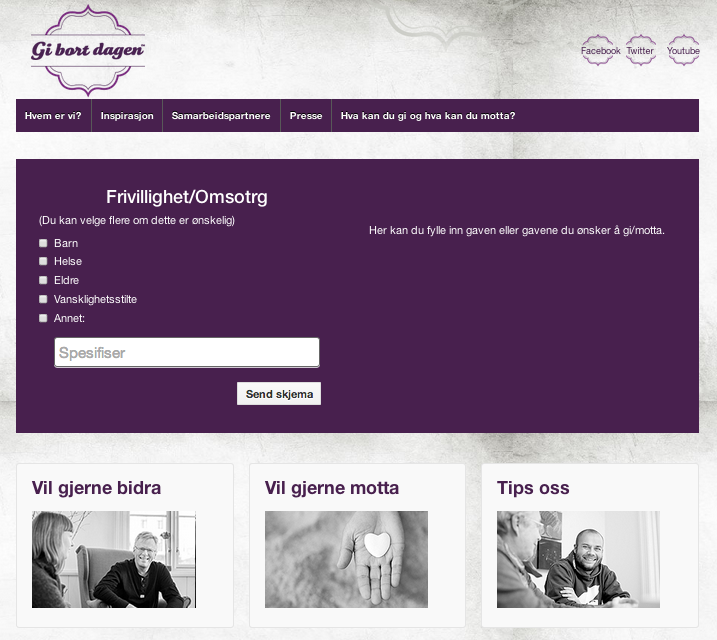
\includegraphics[clip=true, width=1 \textwidth,
trim=0cm 0cm 0cm 0cm]{spesifisertema.png}
\captionof{figure}{Spesifisering av tema ved valg av frivillighet/omsorg}
\label{fig:spesifisertema}
\end{center}

Dersom brukeren krysser av for frivillighet/omsorg i steg 3 vil skjermbildet i figur \ref{fig:spesifisertema} vises. Her skal brukeren nå velge om det er spesifikke temaer innenfor frivillighet og omsorg bedriften helst vil bidra med eller motta. Temaer bedriften kan velge mellom er barn, helse, eldre, vanskelighetsstilte og annet. Når brukeren har huket av de aktuelle temaene må han/hun trykke på “Send skjema” for å komme videre.\\

\newpage

{\bf Steg 4.2:} Spesifiser gave
\begin{center}
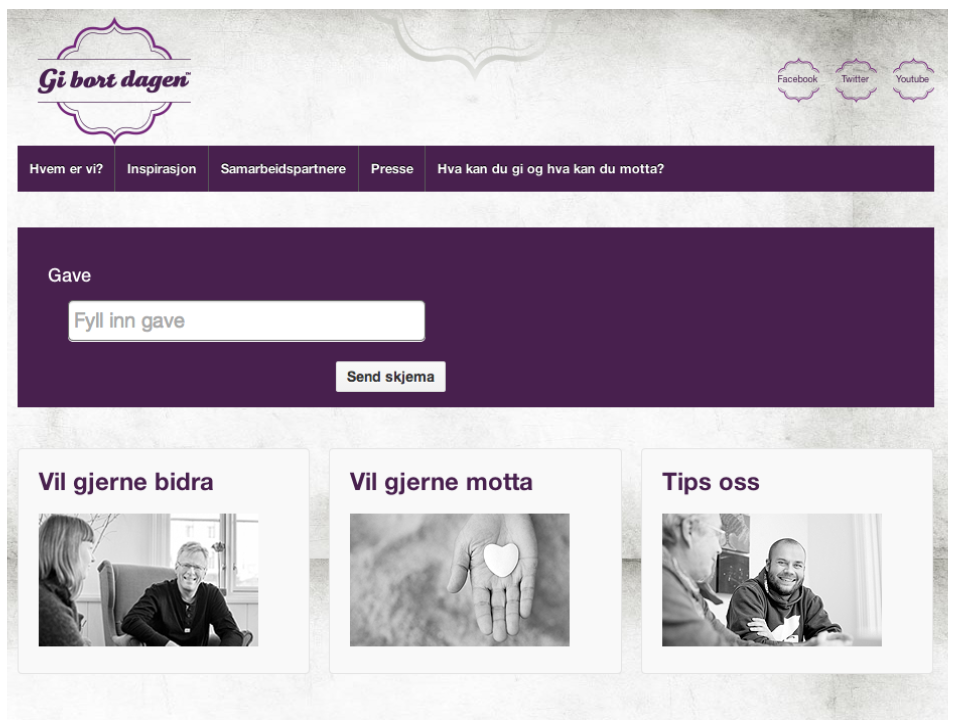
\includegraphics[clip=true, width=1 \textwidth,
trim=0cm 0cm 0cm 0cm]{gave.png}
\captionof{figure}{Spesifisering av gave i prototypen}
\label{fig:gave}
\end{center}
Dersom brukeren har valgt gave i steg 3 består dette steget av å skrive inn hvilken gave dette er i en tekstboks. Når brukeren har gjort dette, må han/hun trykke på ``Send skjema'' for å komme videre til neste steg.\\

\newpage

{\bf Steg 4.3:} Spesifiser tema innenfor kompetanse/kursing
\begin{center}
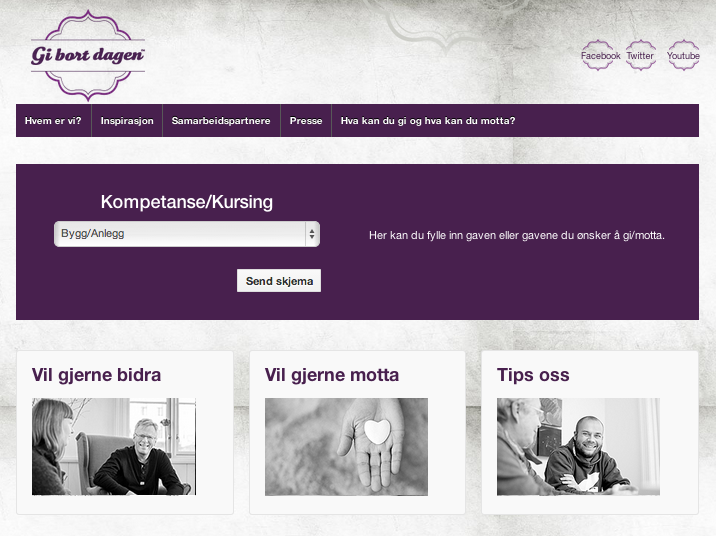
\includegraphics[clip=true, width=1 \textwidth,
trim=0cm 0cm 0cm 0cm]{kompetanse.png}
\captionof{figure}{Spesifisering av type kompetanse/kursing i prototypen}
\label{fig:kompetanse}
\end{center}

Dersom brukeren har valgt kompetanse/kursing i steg 3, må han/hun i dette steget velge type kompetanse/kursing firmaet ønsker å bidra med eller motta fra en nedtrekksmeny. Brukeren sendes vider til neste steg ved å trykke på ``Send skjema''.\\

\newpage

{\bf Steg 5:} Finn en match
Dette steget omhandler å gå gjennom lista med potensielle matcher som kommer opp basert på parameterne brukeren har valgt. Ved å trykke på et spesifikt element i lista vil du få opp mer informasjon om bedriften/organisasjonen som f.eks. kontaktperson, geografisk beliggenhet, beskrivelse av bedriften og hva de har ønsket å gi eller motta. Basert på denne lista må brukeren finne den matchen de ønsker og dermed kontakte kontaktpersonen på telefon eller epost for å avtale nærmere samarbeid.\\
\begin{center}
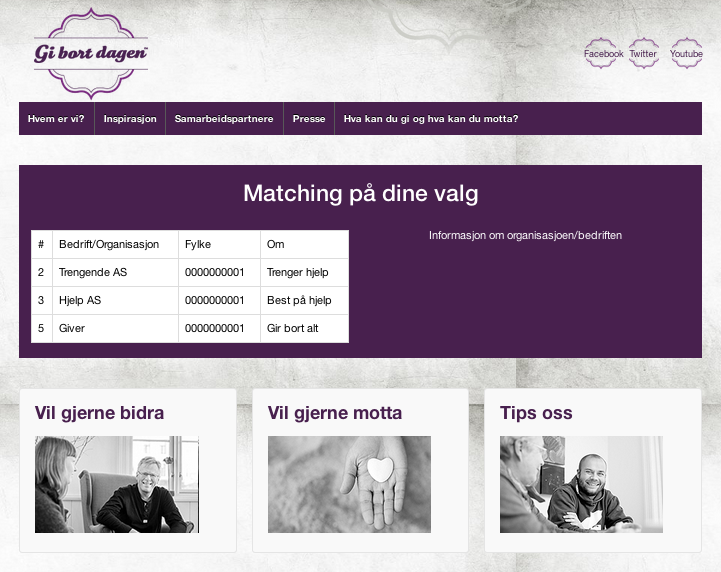
\includegraphics[clip=true, width=1 \textwidth,
trim=0cm 0cm 0cm 0cm]{match.png}
\captionof{figure}{Prototypens liste over potensielle matcher}
\label{fig:match}
\end{center}

Dette utgjør det siste steget i koblingsprosessen i vår prototype. Det er mye utvidet funksjonalitet som kunne vært relevant og ønskelig, og de viktigste punktene presenteres i seksjon 8; Videre arbeid.\\

\section{Presentasjon av koblingslogikken}
Tanken rundt koblingsagenten er som sagt at den skal være enkel, robust og skalerbar. Slik prosjektet ble presentert fra Marianne Daniel sin side, så var det ikke nødvendig med en avansert koblingsagent fordi man kan koble på parametere som er boolske, altså sanne eller usanne.\\

Etter møtet med Marianne ble det enighet om at vi skulle ta utgangspunkt i det allerede eksisterende skjemaet man fyller ut for å bli giver eller mottaker i dag, og lage en koblingsagent på bakgrunn av denne informasjonen. I og med at vi skulle lage en prototype for å vise hvor enkelt man kan koble en giver og mottaker på deres ønsker, så valgte vi å gjøre det så enkelt og oversiktlig som mulig. Vi hadde derfor en MySQL database i bakgrunnen som kunne lagre alle dataene som brukeren la inn om en giver eller mottaker. Dette for å lettere kunne hente ut data om brukere (mottakere/givere) man skulle kobles opp mot etter at man var registrert. Som vist i kapittel \ref{chapter:forslag} er hele prosessen, fra man registrerer seg til man er koblet med en giver/mottaker, skjemabasert. Det vil si at man følger en logisk gang i systemet for å fylle ut nødvendig informasjon og for å kunne matche to bedrifter eller organisasjoner til slutt. Dette gjør prosessen intuitiv for brukerne, samtidig som det sikrer at systemet mottar nødvendig data for å finne gode koblinger.\\

Ved en kobling vil koblingsagenten ta all informasjon om eksisterende bruker, den som registrerer seg, og koble på det man kaller ``fullstendig match''. Det vil si at brukeren bare vil få opp treff på andre brukere som har akkurat de samme valgte parameterne og kriteriene som seg selv. Dette var et valg vi tok fordi vi ville vise hvordan konseptet med en koblingsagent fungerer og ikke gjøre det for avansert i forhold til tiden vi hadde til rådighet i prosjektet. Når det er sagt så har vi lagt opp systemet slik at det ikke skal så mye arbeid til for å koble på det man kaller ``delvis match''. Dette vil si at man kan koble på alle eller noen av de samme parameterne eller kriteriene. Her er det også ønskelig at man kan få opp en prioritert liste basert på ``beste match'' hvor parameteret fylke blir høyest prioritet. ``Best match'' tilsvarer altså den bedriften som har flest identiske parametere med den aktuelle bedriften. Til slutt er det likevel opp til brukeren å velge hvilken bedrift/organisasjon brukerens bedrift vil kobles med.
